%!TEX root = ../Masterthesis.tex
\chapter{System Evaluation}
\section{Image processing performance}
The image  processing of the camera frames on the raspberry can be a significant bottleneck for the system. Real time evaluation demands the processing time of a frame to be in the range of the time of the camera FPS. With the current system setup running at 30fps, this means that the image processing time, containing frame readout and downstream processing of the images, has to be done in about $1/30s$ or 33 ms to achieve "real time" processing.\\ 
The first prototype implementation with \textit{OpenCV} in \textit{Python} showed, that this speed was reachable when only tracking one color. The implementation reached around 30-40 ms processing time when scanning whole images every time. An implementation of an \textit{"Region of interest"} feature\todo {messwerttabelle}  broke down the processing time to around 30 ms for a single color. The downside of the implementation was revealed when implementing the other 4 colors needed to do a full five finger tracking. This approach ramped-up up processing time to around 100 ms per frame, making this solution run at 10 FPS.\\ 
The sequential algorithm also showed another design flaw. When not utilizing the ROI approach, the algorithm would scan the whole grabbed camera frame for each color to create the corresponding threshold map. The \textit{OpenCV} color threshold methods are designed to only search for one color threshold at the time, therefore needing this procedure. One solution option is the already mentioned ROI usage. This solution would furthermore benefit from a multi threaded implementation, as we are not manipulating the original image. Parallel memory readout is not a problem and the generated mask can be saved separately.\\
\\
Another approach which could help speed up the process is implementing an own method for thresholding the grabbed frame with the possibility to do all the needed color thresholds in one image loop. With this solution, the overhead would be reduced by 4 image iterations, thresholding operations would stay the same as these still have to be run on each pixel. The output of this method would then return the 5 needed threshold mask for further processing.\\
Another performance issue that arose from the first prototype was that the input camera frames came RGB coded. For better options of color separations, the image was  initially converted into HSV colorspace. This operation turned out to be second longest operation after frame grabbing. Testing of the cameras showed that the color segmentation in the original RGB images of the cameras are good enough for the used test colors, causing this step to be omitted and shaving off several milliseconds of processing time\todo{insert time}.
The rest of the processing steps were lying in the sub millisecond range and are therefore not as valuable for performance optimization.
The results from this prototype showed, that the \textit{OpenCV-Python} combination is not suitable for reaching the 30 ms target time. \textit{Python} is not a very performant language in this area. The OpenCV library used by python is actually just the ported version of the C code library with bindings for python. As \textit{C} and \textit{C++} are more hardware near and therefore more performant, the second prototype implementation was done in \textit{C++}. The usage of \textit{C++} as the programming language provides more control over memory management and therefore reduces unnecessary memory data copies as these can be handled by pointers to memory locations.\\
\todo{test image correction time}
The ported version of the Python code to\textit{ C+}+ initially showed similar performance measurements when using the sequential approach. This was to be expected, as it is the same code the python bindings are using. Further investigation into code timings showed, that another bottleneck was the image optimization feature which applied an erosion an dilation to remove high frequency noise in the image. This operation brought the time up to 100 ms processing time when processing the whole frame area, making the algorithm  not usable for "real time" application. Removing this feature brought a major speed up in processing time. 
Furthermore, the implementation of a thread pool, which handles all the color detection jobs, brought down the calculation time for 5 colors to around 120-140 ms. Although these times are still not usable for real time, it brought a significant performance boost.

Test of using lower resolution than 640x480 showed that the calculation time reduced furthermore. This indicated that the ROI idea would be feasible for  further performance optimization. A test at a frame resolution of 320x240 pixels reduced the processing time for all five colors to below 10 ms.\\

Utilization of the knowledge from these tests led to the implementation of the aforementioned "region of interest" feature (see Figure \ref{c++ work flow map}).
The first frame is analyzed as a whole frame, optimally resulting in the detection of a marker. As the marker detection creates a rectangle around the tracked area, we already have the coordinates for the ROI and only have to add an offset to this area. This value of the offset has to be set high enough to ensure that in the following frame, the tracking marker is still contained in the ROI. It also has to be ensured, that the generated ROI is clamped to the frame dimensions. If not doing so, parts of the readout are can be located outside of the image plane, causing readout errors when used for the subsequent frame. The following frames will then be processed with the input of the ROI, selecting only the defined section of the image and updating the ROI with the new data for that frame.

As already mentioned in the conceptional phase to lighting of the tracking area is a major factor. Variations of lighting intensity and color temperature cause the color of the trackers to shift their color. This can cause a fluctuation in the calculated tracker positions, as the defined color threshold ranges are kept as small as possible to achieve a clean separation of the tracker colors and reduce unwanted noise. 





\begin{figure}[H]
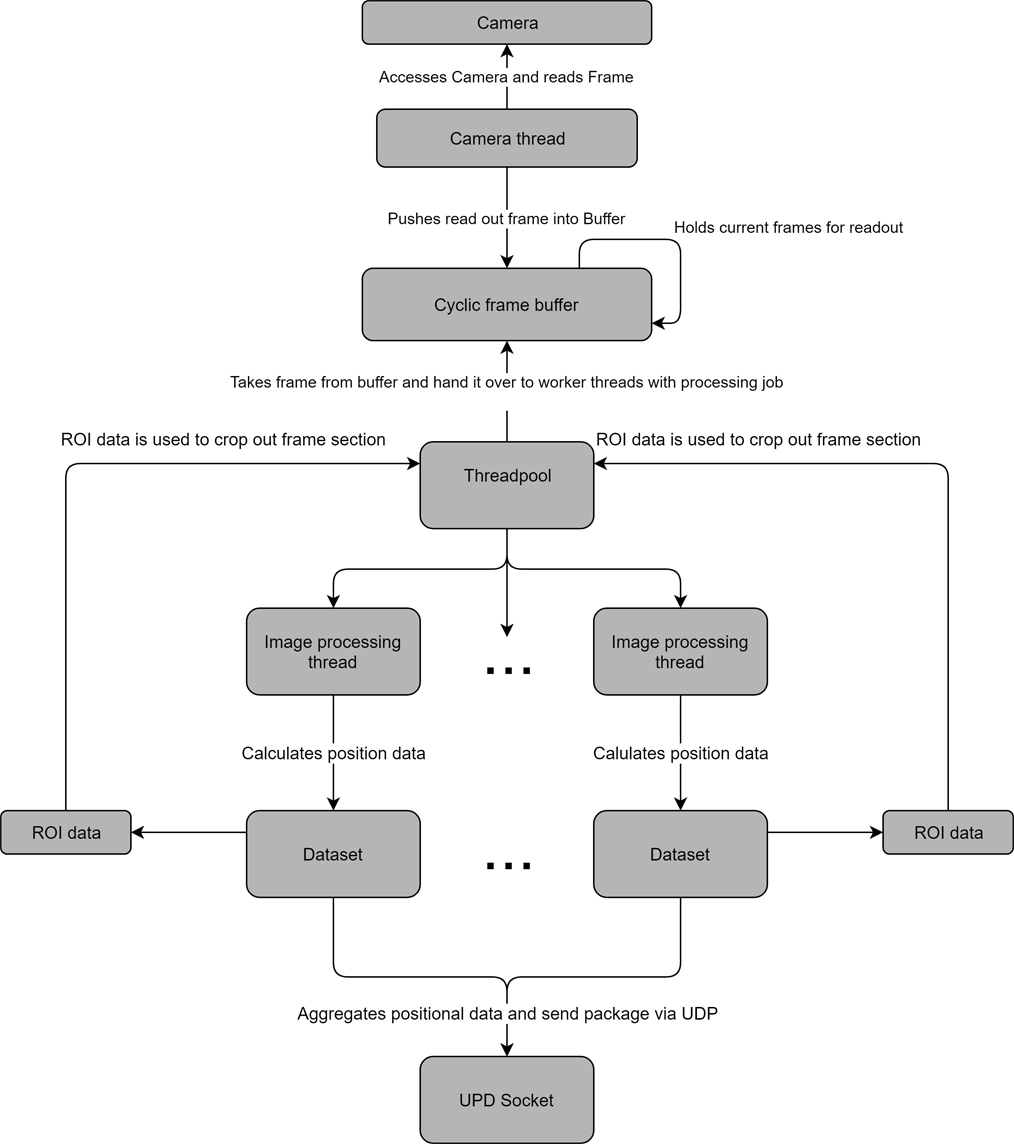
\includegraphics[width=\textwidth]{images/pi_workflow_500.jpg}
\caption{Work flow of the C++ implementation with thread pool solution and ROI}
\label{c++ work flow map} 
\end{figure}
\begin{table}[]
\centering
\caption{My caption}
\label{my-label}
\begin{tabular}{|l|l|l|l|l}
\cline{1-4}
Timings in ms        & \begin{tabular}[c]{@{}l@{}}Python Single Thread \\ without ROI\end{tabular} & \begin{tabular}[c]{@{}l@{}}C++ Single Thread \\ without ROI\end{tabular} & \begin{tabular}[c]{@{}l@{}}C++ Single Threadpool \\ Thread with ROI\end{tabular} &  \\ \cline{1-4}
Frame Reading        &                                                                             &                                                                          &                                                                                  &  \\ \cline{1-4}
HSV Conversion       & \multicolumn{1}{c|}{50.852}                                                 & \multicolumn{1}{c|}{41.125}                                              & omitted                                                                          &  \\ \cline{1-4}
Image Blur          &                                                                             & \multicolumn{1}{c|}{147.239}                                             & 
varies with ROI size &  \\ \cline{1-4}
Mask erode/dilate   &                                                                             & \multicolumn{1}{c|}{165.663}                                             & varies with ROI size &  \\ \cline{1-4}
Color Threshold      &                                                                             & \multicolumn{1}{c|}{14.686}                                              &                                                                                  &  \\ \cline{1-4}
Position Calculation &                                                                             &                                                                          &                                                                                  &  \\ \cline{1-4}
                     &                                                                             &                                                                          &                                                                                  &  \\ \cline{1-4}
ROI Readout          &                                                                             &                                                                          &                                                                                  &  \\ \cline{1-4}
\end{tabular}
\end{table}






 